\documentclass[12pt]{article}
\usepackage{fullpage}
\usepackage{titlesec}
\usepackage{tikz}
\usepackage{amsfonts,amssymb}
\usepackage{amsmath}
\usepackage{comment}
\usetikzlibrary{automata, positioning}
\relpenalty=9999
\binoppenalty=9999

\begin{document}
\pagestyle{plain}
\titleformat{\subsection}[runin]
  {\normalfont\large\bfseries}{\thesubsection}{1em}{}
\titleformat{\subsubsection}[runin]
  {\normalfont\large\bfseries}{\thesubsubsection}{1em}{}

\section*{Problem 3a.}

Consider the following randomized algorithm for this problem. Toss a fair coin
for each vertex $v\in V$, if the coin is heads, place $v$ in $U$, otherwise
place $v$ in $W$. Output $U$ and $W$ as the partition of $V$. Then an edge
$(u,w)$ is in the cut C returned by the algorithm if $u\in U$ and $w \in W$.
Let $X_i$ be a binary random variable such that $X_i = 1$ if an edge
$i = (u,w) \in C$ and $X_i = 0$ otherwise. The probability that an edge $i$
is in the cut then is
$$\textbf{Pr}[X_i = 1] = \textbf{Pr}[u \in U \text{ and } w\in W]$$
Since any two edges $u \neq w$ are placed into $U$ and $W$ independently at
random: $$\textbf{Pr}[X_i = 1] = \textbf{Pr}[u \in U]\cdot\textbf{Pr}[w\in W] =
\frac{1}{2}\cdot\frac{1}{2} = \frac{1}{4}$$
Since $X_i$ are binary random variables:
$$\textbf{E}[X_i] = \textbf{Pr}[X_i = 1] = \frac{1}{4}$$
By linearity of expectation:
$$\textbf{E}[X] = \sum^m_{i=1} \textbf{E}[X_i] = \frac{m}{4}$$
Since the upper bound on the optimum solution for a Directed MAX-CUT problem is
$m$ this algorithm returns a 4-approximate solution in expectation.

\section*{Problem 3b.}
For each vertex $v_i \in V$ let $x_i = 1$ if $v_i \in U$ and $x_i = 0$ if
$v_i \in W$. Then for each edge $(i,j) \in E$, $z_{ij}$ can only take a positive,
non-zero value if $v_i \in U$ and $v_j \in W$. If $v_i \in W$ or $v_j \in U$
then one of the first two conditions in the integer linear program will cause
$z_{ij} = 0$. Therefore, the maximation of all $z_{ij}$ occurs only when the number
of edges of the form $(i,j)$ such that $v_i \in U$ and $v_j \in W$ is maximized,
which is exactly the maximum directed cut problem. Specifically the maximization
of $z_{ij}$'s will cause $z_{ij} = 1$ when $(i,j) \in C$ and $z_{ij} = 0$
otherwise. Therefore the summation of all $z_{ij}$'s will be eqaul to the
maximum directed cut in $G$.

\section*{Problem 3c.}
In the LP relaxation of the integer linear program, we can always assign each
$x_i = \frac{1}{2}$ and subsequently each $z_{ij} = \frac{1}{2}$ without
breaking any of the conditions of the linear program, thus making
$\frac{|E|}{2}$ a feasible solution for the linear program and a lower bound on
its maximization for an instance of the problem. Now consider the following
graph:
\newline
\begin{center}
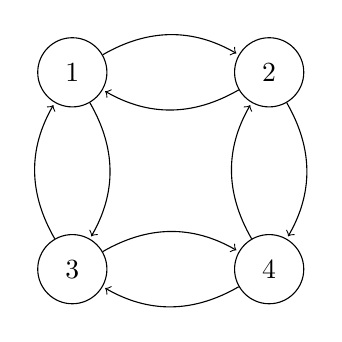
\begin{tikzpicture}[shorten >=1pt, node distance=2.5cm, on grid, auto]
  \node[state] (1) {$1$};
  \node[state] (2) [right=of 1] {2};
  \node[state] (3) [below=of 1] {3};
  \node[state] (4) [below=of 2] {4};
  \path[->]
  (1) edge [bend left] (2)
  (2) edge [bend left] (1)
  (1) edge [bend left] (3)
  (3) edge [bend left] (1)
  (2) edge [bend left] (4)
  (4) edge [bend left] (2)
  (3) edge [bend left] (4)
  (4) edge [bend left] (3)
  ;
\end{tikzpicture}
\end{center}
Since $|E| = 8$, the LP relaxation of the integer linear program will return
a maximum directed cut size of at least $4$ but the graph has a maximum
directed cut of size $2$ thus showing the integrality gap of the relaxation is
at least $2$.

\section*{Problem 3d.}

\end{document}
